\documentclass[a4j,11pt,dvipdfmx]{jsarticle}
\usepackage{float}
\usepackage{array}
\usepackage{titlesec}
\usepackage[dvipdfmx]{graphicx}
\usepackage{graphicx}
\usepackage{url}
\usepackage{listings,jvlisting} 

\lstset{
  basicstyle={\ttfamily},
  identifierstyle={\small},
  commentstyle={\smallitshape},
  keywordstyle={\small\bfseries},
  ndkeywordstyle={\small},
  stringstyle={\small\ttfamily},
  frame={tb},
  breaklines=true,
  columns=[l]{fullflexible},
  numbers=left,
  xrightmargin=0zw,
  xleftmargin=3zw,
  numberstyle={\scriptsize},
  stepnumber=1,
  numbersep=1zw,
  lineskip=-0.5ex
}

\titleformat*{\section}{\bfseries}
\titleformat*{\subsection}{\bfseries}

\makeatletter
  \renewcommand{\section}{%
    \@startsection{section}{1}{\z@}%
    {0.4\Cvs}{0.1\Cvs}%
    {\normalfont\headfont\raggedright}}
\makeatother

\makeatletter
  % sectionの下マージンを小さく
  \renewcommand{\subsection}{%
    \@startsection{subsection}{1}{\z@}%
    {0.1\Cvs}{0.1\Cvs}%
    {\normalfont\headfont\raggedright}}
\makeatother

\renewcommand{\thesubsection}{\thesection-\arabic{subsection}.}


%---------------------------------------------------
% ページの設定
%---------------------------------------------------
\setlength{\textwidth}{160truemm}
\setlength{\textheight}{250truemm}
\setlength{\topmargin}{-10.5truemm}
\setlength{\oddsidemargin}{0.5truemm}

\setlength{\headheight}{0truemm}
\setlength{\parindent}{1zw}
\newcolumntype{b}{!{\vrule width 1pt}}
\newcommand{\bhline}{\noalign{\hrule height 1pt}}   


\begin{document}
%提出日: \today

\begin{flushleft}

\large{\textbf{作業ログ}} 
\hspace{0.5em}
\normalsize{チーム40}
\\

\normalsize{
\vspace{1em}
\textbf{報告者：} 24G1136{\hspace{1em}}山口{\hspace{0.5em}}侑希 \\
\vspace{1em}
\textbf{報告日：} \today   （{第6週目}）\\
\vspace{1em}
\textbf{プロジェクト名：}マジカル☆観覧車
}
\end{flushleft}

%%%%%%%%%%%%%%%%%%%%%%%%%%%%%%%%%%%%%%%%%%%%%%%%%
\hrulefill
\section{進捗サマリー（要約）}
%

\begin{itemize}
  \item 全体進捗率:{7}[\%]

  %達成 遅延 前倒し
  \item マイルストーン達成状況:{遅延}

  \item 主要成果:
  \begin{itemize}
    \item {成果名1} 部品機材調達
  \end{itemize}

  \item 重大課題（影響度:高）:
  \begin{itemize}
    % {課題} \hspace{1em} {影響具合(一言)}
    \item {課題} \hspace{1em} {なし}
  \end{itemize}
\end{itemize}

%%%%%%%%%%%%%%%%%%%%%%%%%%%%%%%%%%%%%%%%%%%%%%%%%
\hrulefill
\section{作業ログ（詳細トラッキング）}
% 画像等がある場合は\ref{}で参照すること

%------------------------------------------------
\subsection{作業ログ概要}
部品調達と設計を行った．
部品調達に関しては，予定である25日より1日多い26日に完了した．

\begin{table}[H]
\begin{tabular}{p{5em}|p{5em} p{5em} p{5em} p{4em} p{7em} p{7em}}
作業項目 & 開始日 & 予定完了日 & 状態 & 進捗率 & 依存関係・\hspace{3em}ブロッカー & コメント \\ \hline\hline
%%%%%%%%%%%%%%%%%%%%%%%
作業1\\
部品調達(指揮) & %作業名
5月22日 & %開始日
5月25日 & %完了予定日
% 未着手 進行中 レビュー中 完了
完了 & %状況
100[\%] & %進捗率
無 & %依存関係・ブロッカー
26日に完了した %コメント（特記事項）
\\ \hline
%%%%%%%%%%%%%%%%%%%%%%%

%%%%%%%%%%%%%%%%%%%%%%%
作業2\\
部品調達(中継機) & %作業名
5月22日 & %開始日
5月25日 & %完了予定日
% 未着手 進行中 レビュー中 完了
完了 & %状況
100[\%] & %進捗率
無 & %依存関係・ブロッカー
26日に完了した %コメント（特記事項）
\\ \hline
%%%%%%%%%%%%%%%%%%%%%%%

%%%%%%%%%%%%%%%%%%%%%%%
作業3\\
観覧車設計・部品用意 & %作業名
5月22日 & %開始日
5月29日 & %完了予定日
% 未着手 進行中 レビュー中 完了
進行中 & %状況
10[\%] & %進捗率
無 & %依存関係・ブロッカー
なし %コメント（特記事項）
\\ \hline
%%%%%%%%%%%%%%%%%%%%%%%
\end{tabular}
\end{table}

%------------------------------------------------
\subsection{日ごとの作業ログ}
%何もしなかった日は記入しなくてよい
\begin{table}[H]
\begin{tabular}{p{5em} | p{4em} p{4em} p{6em} p{6em} p{3em} p{4em} p{5em}}
日付 & 作業項目 & 作業時間 & 開始時の状態 & 終了時の状態 & 進捗率 & 課題発生 & コメント \\ \hline\hline

%%%%%%%%%%%%%%%%%%%%%%%
5月22日 & %日付 上記と同じであれば未記入
作業1 & %作業項目
0h & %作業時間
% 未着手 進行中 レビュー中 完了
未着手 & %開始時の状態
% 未着手 進行中 レビュー中 完了
未着手 & %終了時の状態
0[\%] & %進捗率
%有 無
無 & %課題発生
- %コメント（特記事項）
\\
%%%%%%%%%%%%%%%%%%%%%%%

%%%%%%%%%%%%%%%%%%%%%%%
 & %日付 上記と同じであれば未記入
作業2 & %作業項目
0h & %作業時間
% 未着手 進行中 レビュー中 完了
未着手 & %開始時の状態
% 未着手 進行中 レビュー中 完了
未着手 & %終了時の状態
0[\%] & %進捗率
%有 無
無 & %課題発生
- %コメント（特記事項）
\\
%%%%%%%%%%%%%%%%%%%%%%%

%%%%%%%%%%%%%%%%%%%%%%%
 & %日付 上記と同じであれば未記入
作業3 & %作業項目
0h & %作業時間
% 未着手 進行中 レビュー中 完了
未着手 & %開始時の状態
% 未着手 進行中 レビュー中 完了
未着手 & %終了時の状態
0[\%] & %進捗率
%有 無
無 & %課題発生
-%コメント（特記事項）
\\
%%%%%%%%%%%%%%%%%%%%%%%

\hline

%%%%%%%%%%%%%%%%%%%%%%%
5月23日 & %日付 上記と同じであれば未記入
作業1 & %作業項目
3h & %作業時間
% 未着手 進行中 レビュー中 完了
未着手 & %開始時の状態
% 未着手 進行中 レビュー中 完了
進行中 & %終了時の状態
30[\%] & %進捗率
%有 無
無 & %課題発生
- %コメント（特記事項）
\\
%%%%%%%%%%%%%%%%%%%%%%%

%%%%%%%%%%%%%%%%%%%%%%%
 & %日付 上記と同じであれば未記入
作業2 & %作業項目
3h & %作業時間
% 未着手 進行中 レビュー中 完了
未着手 & %開始時の状態
% 未着手 進行中 レビュー中 完了
進行中 & %終了時の状態
30[\%] & %進捗率
%有 無
無 & %課題発生
- %コメント（特記事項）
\\
%%%%%%%%%%%%%%%%%%%%%%%

%%%%%%%%%%%%%%%%%%%%%%%
 & %日付 上記と同じであれば未記入
作業3 & %作業項目
0h & %作業時間
% 未着手 進行中 レビュー中 完了
未着手 & %開始時の状態
% 未着手 進行中 レビュー中 完了
進行中 & %終了時の状態
0[\%] & %進捗率
%有 無
無 & %課題発生
-%コメント（特記事項）
\\
%%%%%%%%%%%%%%%%%%%%%%%

\hline

%%%%%%%%%%%%%%%%%%%%%%%
5月24日 & %日付 上記と同じであれば未記入
作業1 & %作業項目
5h & %作業時間
% 未着手 進行中 レビュー中 完了
進行中 & %開始時の状態
% 未着手 進行中 レビュー中 完了
レビュー中 & %終了時の状態
70[\%] & %進捗率
%有 無
無 & %課題発生
注文完了 %コメント（特記事項）
\\
%%%%%%%%%%%%%%%%%%%%%%%

%%%%%%%%%%%%%%%%%%%%%%%
 & %日付 上記と同じであれば未記入
作業2 & %作業項目
5h & %作業時間
% 未着手 進行中 レビュー中 完了
進行中 & %開始時の状態
% 未着手 進行中 レビュー中 完了
レビュー中 & %終了時の状態
70[\%] & %進捗率
%有 無
無 & %課題発生
注文完了 %コメント（特記事項）
\\
%%%%%%%%%%%%%%%%%%%%%%%

%%%%%%%%%%%%%%%%%%%%%%%
 & %日付 上記と同じであれば未記入
作業3 & %作業項目
0h & %作業時間
% 未着手 進行中 レビュー中 完了
進行中 & %開始時の状態
% 未着手 進行中 レビュー中 完了
進行中 & %終了時の状態
0[\%] & %進捗率
%有 無
無 & %課題発生
- %コメント（特記事項）
\\
%%%%%%%%%%%%%%%%%%%%%%%

\hline

%%%%%%%%%%%%%%%%%%%%%%%
5月25日 & %日付 上記と同じであれば未記入
作業1 & %作業項目
0h & %作業時間
% 未着手 進行中 レビュー中 完了
レビュー中 & %開始時の状態
% 未着手 進行中 レビュー中 完了
レビュー中 & %終了時の状態
80[\%] & %進捗率
%有 無
無 & %課題発生
- %コメント（特記事項）
\\
%%%%%%%%%%%%%%%%%%%%%%%

%%%%%%%%%%%%%%%%%%%%%%%
 & %日付 上記と同じであれば未記入
作業2 & %作業項目
0h& %作業時間
% 未着手 進行中 レビュー中 完了
レビュー中 & %開始時の状態
% 未着手 進行中 レビュー中 完了
レビュー中 & %終了時の状態
80[\%] & %進捗率
%有 無
無 & %課題発生
- %コメント（特記事項）
\\
%%%%%%%%%%%%%%%%%%%%%%%

%%%%%%%%%%%%%%%%%%%%%%%
 & %日付 上記と同じであれば未記入
作業3 & %作業項目
1h & %作業時間
% 未着手 進行中 レビュー中 完了
進行中 & %開始時の状態
% 未着手 進行中 レビュー中 完了
進行中 & %終了時の状態
5[\%] & %進捗率
%有 無
無 & %課題発生
- %コメント（特記事項）
\\
%%%%%%%%%%%%%%%%%%%%%%%

\hline

%%%%%%%%%%%%%%%%%%%%%%%
5月26日 & %日付 上記と同じであれば未記入
作業1 & %作業項目
0h & %作業時間
% 未着手 進行中 レビュー中 完了
レビュー中 & %開始時の状態
% 未着手 進行中 レビュー中 完了
完了 & %終了時の状態
100[\%] & %進捗率
%有 無
無 & %課題発生
- %コメント（特記事項）
\\
%%%%%%%%%%%%%%%%%%%%%%%

%%%%%%%%%%%%%%%%%%%%%%%
 & %日付 上記と同じであれば未記入
作業2 & %作業項目
0h & %作業時間
% 未着手 進行中 レビュー中 完了
レビュー中 & %開始時の状態
% 未着手 進行中 レビュー中 完了
完了 & %終了時の状態
100[\%] & %進捗率
%有 無
無 & %課題発生
- %コメント（特記事項）
\\
%%%%%%%%%%%%%%%%%%%%%%%

%%%%%%%%%%%%%%%%%%%%%%%
 & %日付 上記と同じであれば未記入
作業3 & %作業項目
2h & %作業時間
% 未着手 進行中 レビュー中 完了
進行中 & %開始時の状態
% 未着手 進行中 レビュー中 完了
進行中 & %終了時の状態
10[\%] & %進捗率
%有 無
無 & %課題発生
- %コメント（特記事項）
\\
%%%%%%%%%%%%%%%%%%%%%%%
\hline
\end{tabular}
\end{table}

%%%%%%%%%%%%%%%%%%%%%%%%%%%%%%%%%%%%%%%%%%%%%%%%%
\hrulefill
\section{課題管理}
% 画像等がある場合は\ref{}で参照すること

\begin{table}[h]
\begin{tabular}{p{5em}|p{7em} p{3em} p{3em} p{7em} p{5em} p{3em}}
課題 & 発生原因 & 影響度 & 優先度 & 対策 & 期限 & 状態 \\ \hline\hline

%%%%%%%%%%%%%%%%%%%%%%%
なし & %課題概要
ー & %発生原因
% 高 中 低
ー & %影響度
% 高 中 低
ー & %優先度
ー & %対策
ー& %期限
%未対応 対応中 解決
ー %状態
\\ \hline
%%%%%%%%%%%%%%%%%%%%%%%

\end{tabular}
\end{table}

\noindent
※影響度=プロジェクトへのインパクト
\vspace{0.5em}

\noindent
※優先度=対応の緊急性



%%%%%%%%%%%%%%%%%%%%%%%%%%%%%%%%%%%%%%%%%%%%%%%%%
\hrulefill
\section{AI利用状況と検証（再現性重視）}
AIの利用はしていない

\ifodd 0
%------------------------------------------------

\subsection{利用内容}
% 
\begin{itemize}
  \item \textbf{利用目的}:{探索}
  
  \item \textbf{入力（プロンプト趣旨）}:
  \begin{itemize}
    % 何をどのように聞いたか
    \item 
  \end{itemize}

  \item \textbf{出力概要}:
  \begin{itemize}
    % 何が得られたのか
    \item 
  \end{itemize}
\end{itemize}

%------------------------------------------------
\subsection{検証方法}
\noindent
※第三者が再現できるレベルで記述

\begin{itemize}
  \item \textbf{検証手法}:
  \begin{itemize}
    % 実験/比較/理論確認など
    \item 
  \end{itemize}

  \item \textbf{参照資料}:
  \begin{itemize}
    % 論文/書籍/公式ドキュメントなど
    \item 
  \end{itemize}

  \item \textbf{検証手段}:
  \begin{enumerate}
    % 何が得られたのか
    \item {検証1}
    \item {検証2}
  \end{enumerate}
\end{itemize}

%------------------------------------------------
\subsection{ファクトチェック結果}

\begin{itemize}
  \item \textbf{一致点}:
  \begin{itemize}
    % 既存知識と整合している部分
    \item 
  \end{itemize}

  \item \textbf{不一致・疑義}:
  \begin{itemize}
    % 差異の内容
    \item 
  \end{itemize}

  \item \textbf{最終判断}:
  \begin{itemize}
    % 採用/保留/破棄
    \item 
  \end{itemize}

  \item \textbf{根拠}:
  \begin{itemize}
    % 資料/理由
    \item 
  \end{itemize}
\end{itemize}
\fi
%%%%%%%%%%%%%%%%%%%%%%%%%%%%%%%%%%%%%%%%%%%%%%%%%
\hrulefill
\section{次回計画}

\begin{itemize}
  \item \textbf{目標}:
  \begin{itemize}
    % タスク内容
    \item {観覧車の設計}
    \item {指揮デバイスと観覧車デバイスの回路設計}
  \end{itemize}

  \item \textbf{達成基準}:
  \begin{itemize}
    % 検証可能な条件
    \item {回路が正常に動作したか}
    \item {観覧車製作の部品が完成したか}
  \end{itemize}

  \item \textbf{期限}:
  \begin{itemize}
    % 日付
    \item {6月2日}
  \end{itemize}
\end{itemize}

%%%%%%%%%%%%%%%%%%%%%%%%%%%%%%%%%%%%%%%%%%%%%%%%%
\hrulefill
\section{その他}
%ない場合は なし と記入
\begin{itemize}
  \item 特記事項：なし
\end{itemize}

%%%%%%%%%%%%%%%%%%%%%%%%%%%%%%%%%%%%%%%%%%%%%%%%%
\ifodd 1 %ない場合は0に変更
\clearpage
\hrulefill
\section{付録}
%必ず説明を記入すること

%作業ログ及び課題管理で関係する場合は
%必ず該当部分に\ref{}で参照すること

%はみ出す場合は\clearpageで改ページすること

\begin{figure}[h]
\centering
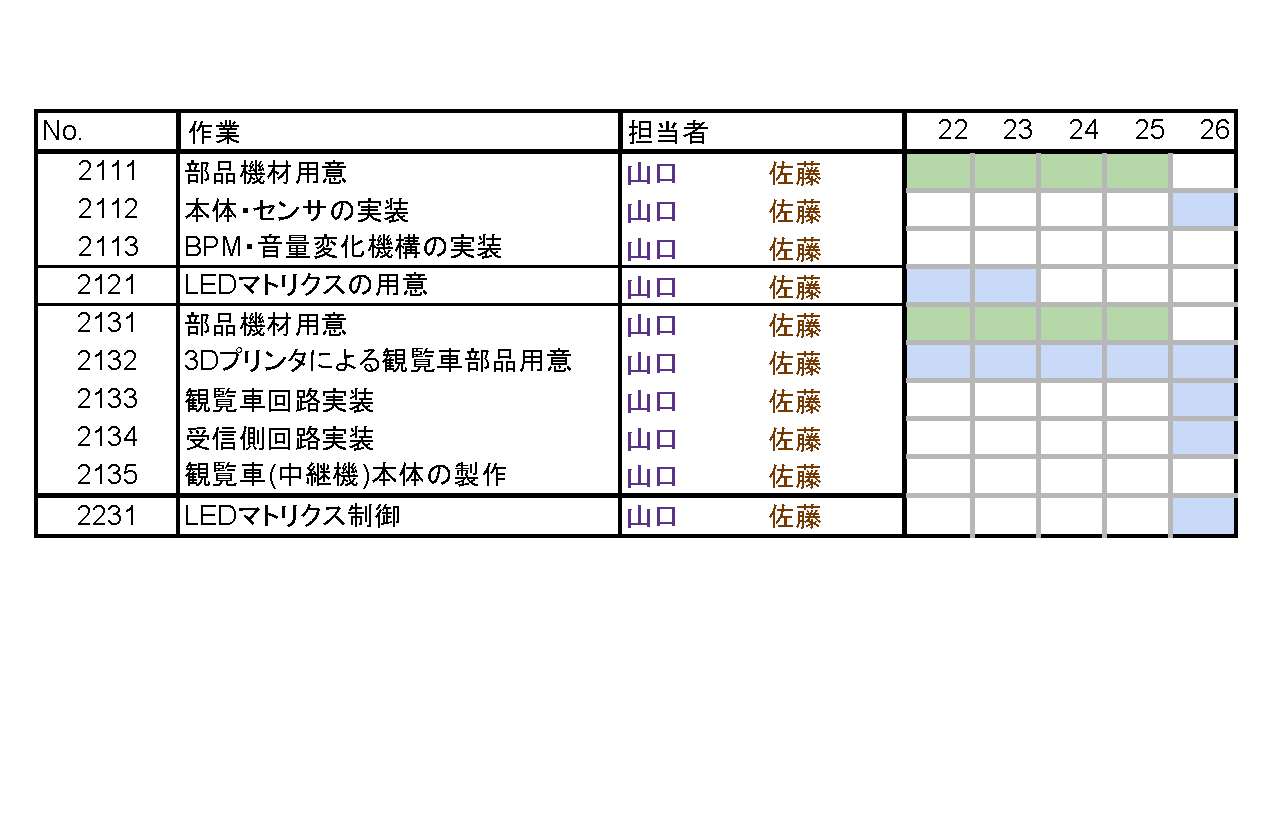
\includegraphics[width=10cm]{Fig/ガント1.pdf} 
\caption{現在のガントチャート}
\label{fig:example}
\end{figure}

\ifodd 0
\begin{table}[h]
\centering
\caption{表の例}
\label{tab:example}
\begin{tabular}{|c|c|c|} \hline
A & B & C \\ \hline
100 & 90 & 60 \\ \hline
\end{tabular}
\end{table}

\fi
%\begin{lstlisting}[caption=example.ino, language=C++, label=lst:ino]
%\end{lstlisting}

\fi
%%%%%%%%%%%%%%%%%%%%%%%%%%%%%%%%%%%%%%%%%%%%%%%%%

\end{document}

